\section{Allocation Across Rounds}
\label{sec:results-alloc}

All results in this section use the calibrated regime of
Chapter~4 and the paired protocol of Section~\ref{sec:protocol}. The
quantity Theorem~\ref{thm:uniform} identifies as governing the outcome,
the accumulated noise variance $\sum_t\sigma_t^2$, is reported alongside every
schedule as a multiple of the uniform minimum, so that the theory's prediction
can be read directly against the measurement.

\subsection{Power-Law Schedules}

We allocate $\rho_t \propto (t+1)^{k}$, normalised to spend $\rho=30$ exactly.
Here $k=0$ is uniform, and $k>0$ places less noise late, which is the direction
predicted by the adaptive-allocation literature. Table~\ref{tab:headroom}
reports $n=20$ paired trials.

\begin{table}[H]
\centering
\caption{Power-law schedules against uniform, $n=20$ paired trials with common
random numbers, $\rho=30$. The variance penalty is $\sum_t\sigma_t^2$ relative
to the uniform minimum. Every significant entry is a loss.}
\label{tab:headroom}
\begin{tabular}{lrrrr}
\toprule
$k$ & Variance penalty & Mean difference & 95\% CI & $p$ \\
\midrule
$-1.0$ & $1.99\times$ & $+0.0023$ & $[-0.0012,+0.0058]$ & 0.19 \\
$+0.5$ & $1.18\times$ & $-0.0018$ & $[-0.0041,+0.0006]$ & 0.13 \\
$+1.0$ & $1.98\times$ & $-0.0045$ & $[-0.0125,+0.0035]$ & 0.25 \\
$+2.0$ & $10.15\times$ & $-0.0214$ & $[-0.0447,+0.0018]$ & 0.069 \\
$+3.0$ & $21.03\times$ & $-0.0539$ & $[-0.0878,-0.0201]$ & \textbf{0.0034} \\
\bottomrule
\end{tabular}
\end{table}

The ordering is monotone in $k$, and every step toward the literature's
prescription is worse, significantly so at the extreme. Only $k=-1$ sits above
uniform, and it is not significant; Section~\ref{sec:frontload} shows that it
does not replicate.

\subsection{A Mild Front-Load}
\label{sec:frontload}

Because $k=-1$ and $k=+1$ carry near-identical variance penalties
($1.99\times$ against $1.98\times$) yet differed in sign, the possibility
remained of a genuine timing effect distinct from the variance term. If such an
effect existed, it could be bought most cheaply at small negative $k$, where the
variance penalty is negligible ($k=-0.25$ costs $1.04\times$). We pre-registered
that test and ran it on disjoint seeds.

\vspace{10pt}

At $n=16$ paired trials the effect is absent: $k=-0.25$ gives $-0.0007$ with
95\% CI $[-0.0018,+0.0003]$, and $k=-1$ does not replicate, moving from
$+0.0023$ to $-0.0013$. \textbf{Any gain from mild front-loading is bounded
above by $+0.0003$ IoU$_{.25}$}, equivalently $0.04\%$ relative, which is the
tightest null in this study. The apparent asymmetry on which the hypothesis
rested was itself noise.

\subsection{Beyond the Power Family}

A power law is a narrow family, and an optimality claim should not rest on it.
Bang-bang schedules, consisting of a run of minimum-noise rounds with the
remaining budget spread over the rest, in both orderings, and random draws from
the budget simplex also lose to uniform, by $-0.047$ to $-0.112$. Early
stopping, spending the whole budget over $T'<T$ rounds and halting, is neutral
at best: the $\sqrt{T}$ averaging gain exactly offsets the
$\sigma\propto\sqrt{T}$ budget cost, measured at $+0.0011$ for $T'=20$ and
$-0.058$ for $T'=8$.

\subsection{One Scalar Explains Everything}

Figure~\ref{fig:variance} plots all 13 allocations against their accumulated
noise variance. A single scalar orders outcomes across three unrelated families:
Spearman $\rho=-0.767$ ($p=0.0022$), and Pearson on log variance $-0.851$
($p=0.00023$). Uniform sits at the minimum, $1.00\times$, and nothing beats it.

\vspace{10pt}

This is the central empirical result. It is stronger than the individual
comparisons because it is a prediction about the \emph{ordering} of unrelated
schedule families from a single closed-form quantity, and that prediction holds
across families that share no structure other than their variance.

\begin{figure}[H]
\centering
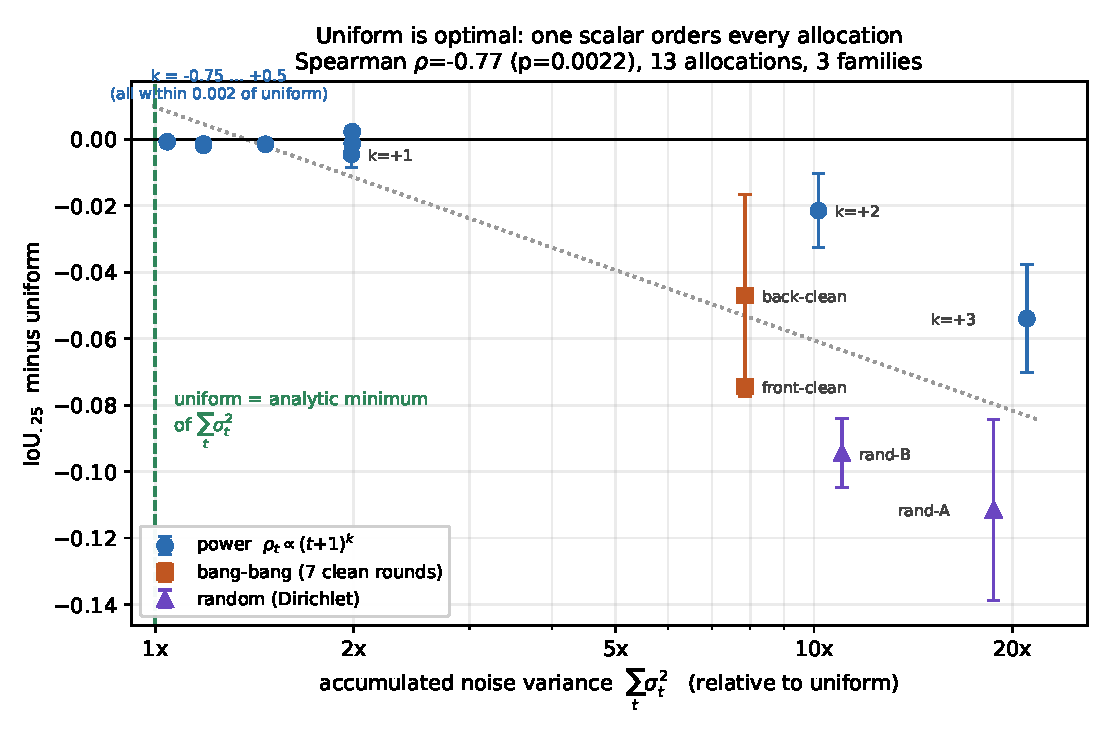
\includegraphics[width=0.9\textwidth]{figC_allocation_variance.pdf}
\caption{Accumulated noise variance $\sum_t\sigma_t^2$ orders every allocation
tested, across power-law, bang-bang and random-simplex families. Uniform is the
analytic minimum.}
\label{fig:variance}
\end{figure}

\subsection{Tight Privacy Budgets}
\label{sec:results-tight}

Theorem~\ref{thm:uniform} assumes utility is smooth and monotone in accumulated
variance, an assumption weakest near the collapse threshold, where outcomes
become bimodal: a run either survives the noise or fails. If any allocation is
to beat uniform, this is where it should happen, because concentrating a tiny
budget into a few usable rounds might rescue a run that spreading it thin would
lose. We therefore ran a pre-specified ladder at $\rho\in\{0.5,2,8\}$ against
truncation depths $T'\in\{3,6,12,25\}$, $n=10$ paired trials, reporting all
outcomes (Table~\ref{tab:tight}).

\begin{table}[H]
\centering
\caption{Truncation against uniform across privacy budgets, $n=10$ paired
trials. Entries are the mean IoU$_{.25}$ difference, with wins out of 10 in
parentheses. $^{*}p<0.05$, $^{**}p<0.01$.}
\label{tab:tight}
\small
\begin{tabular}{lrrr}
\toprule
$\rho$ (uniform $\sigma$) & $T'=12$ & $T'=6$ & $T'=3$ \\
\midrule
$0.5$ ($\sigma=14.1$) & $+0.036$ (5/10) & $+0.040$ (4/10) & $-0.050$ (4/10) \\
$2.0$ ($\sigma=7.07$) & $-0.025$ (3/10) & $-0.034$ (3/10) & $-0.123^{*}$ (2/10) \\
$8.0$ ($\sigma=3.54$) & $-0.022$ (2/10) & $-0.039^{*}$ (1/10) & $-0.128^{**}$ (1/10) \\
\bottomrule
\end{tabular}
\end{table}

No allocation significantly beats uniform at any budget, and every significant
entry is a loss. At $\rho=0.5$ the point estimates turn positive, but the win
counts of 4/10 and 5/10 are coin flips: the positive mean comes from a few large
asymmetric outliers, occasions on which concentrating the budget rescued a run
that uniform lost, rather than from consistent superiority.

\vspace{10pt}

What does change with budget is the size of the penalty for deviating, which
shrinks monotonically as the budget tightens, with a slope against $\log\rho$ of
$-0.021$ to $-0.029$ across the three truncation depths. The theorem's
smoothness assumption therefore does measurably weaken toward the cliff, exactly
as anticipated, but never enough to reverse the ordering. Reporting that
gradient inside a null result is the honest characterisation: uniform's margin
erodes at tight budgets and is never overturned.

\vspace{10pt}

Crucially, the paired standard deviation grows faster than the effect,
from $0.060$ at $\rho=8$ to $0.103$ at $\rho=2$ and $0.173$ at $\rho=0.5$, so
the best candidate gain of $+0.040$ sits at less than a quarter of the noise in
the very signal an agent would have to learn from. Resolving it would require
$n=73$, roughly 28 hours of computation, and with 4/10 wins that is very likely
chasing noise. \textbf{Even were the gain real, it would be unlearnable.}
Figure~\ref{fig:crossover} shows both panels.

\begin{figure}[H]
\centering
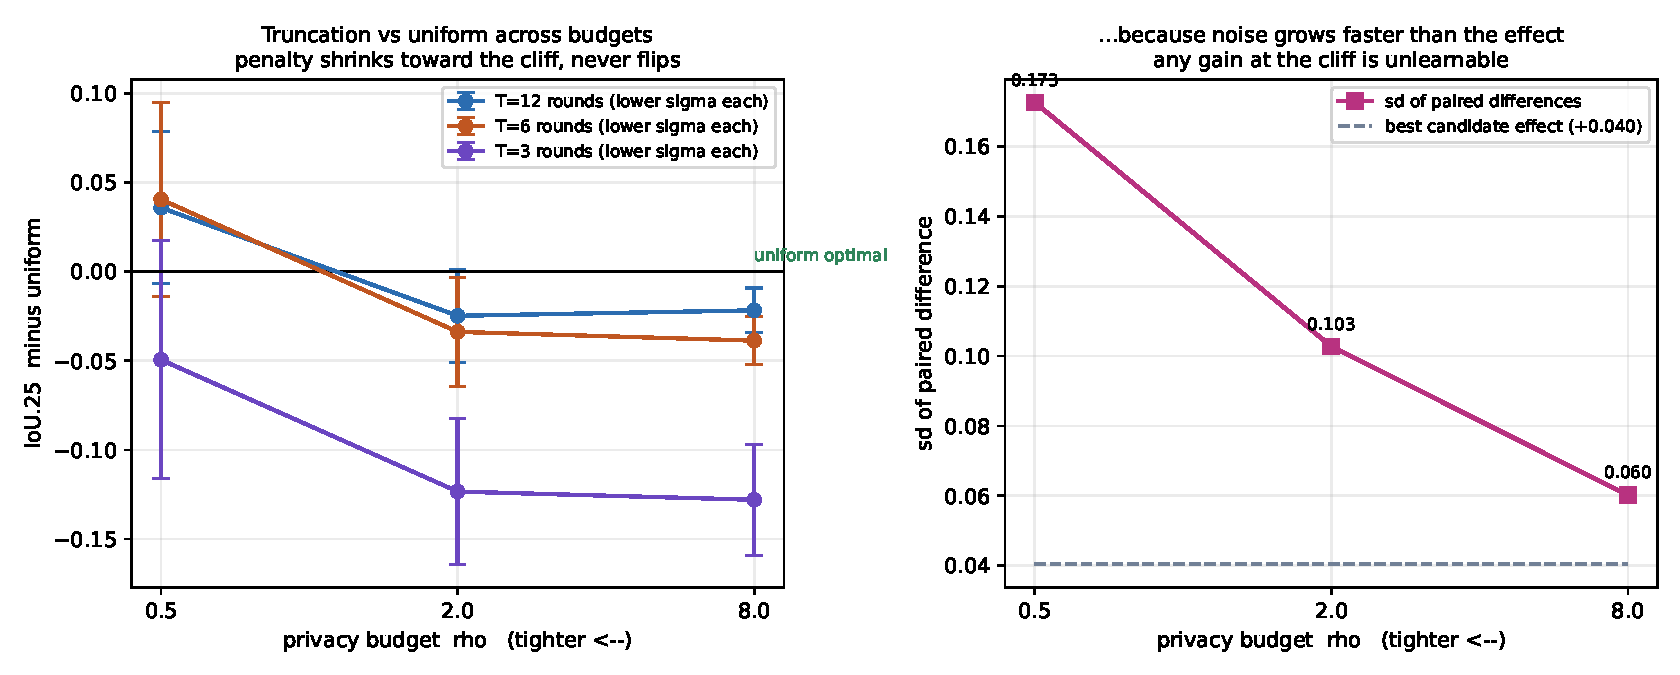
\includegraphics[width=\textwidth]{figD_budget_crossover.pdf}
\caption{Left: the penalty for deviating from uniform shrinks toward the
collapse threshold but never flips sign. Right: paired-difference noise grows
faster than the candidate effect.}
\label{fig:crossover}
\end{figure}

\subsection{The Learned Allocator in Practice}
\label{sec:drl-practice}

Sections~\ref{sec:results-alloc}--\ref{sec:results-tight} bound the class of
fixed schedules, and Section~\ref{sec:consequence} argues that the published
agent belongs to that class because its state carries no model feedback. That
argument is structural. It is worth also running the agent, and we do.

\vspace{10pt}

We trained the DDPG agent with parameter sharing and value decomposition, as
described by \citeauthor{ChenAdaptivePrivacyMARL}
\cite{ChenAdaptivePrivacyMARL}, and compared it against the uniform, exponential
and arithmetic baselines used in that work. Comparisons are paired, with all
four arms sharing one initialisation per trial, over $n=8$ trials, and every
point is scored on a held-out validation set that no client trains on.
Table~\ref{tab:drl} reports final accuracy and Figure~\ref{fig:drlmap} the
trajectories.

\begin{table}[H]
\centering
\caption{The learned allocator against the baselines it was designed to beat.
Final mAP@0.5 on held-out data, $n=8$ paired trials, mean $\pm$ standard
deviation; differences are DRL minus baseline.}
\label{tab:drl}
\small
\begin{tabular}{lcrrr}
\toprule
Method & Final mAP@0.5 & Difference & 95\% CI & Wins \\
\midrule
DRL (learned) & $0.8629\pm0.0606$ & --- & --- & --- \\
Uniform & $0.9060\pm0.0483$ & $-0.0431$ & $[-0.0997,+0.0136]$ & 3/8 \\
Exponential & $0.8738\pm0.0666$ & $-0.0109$ & $[-0.0674,+0.0456]$ & 4/8 \\
Arithmetic & $0.8931\pm0.0761$ & $-0.0302$ & $[-0.0761,+0.0157]$ & 3/8 \\
\bottomrule
\end{tabular}
\end{table}

The agent does not beat any of the three baselines. Every point estimate is
negative, and it loses to uniform by $-0.0431$ with 3 wins in 8 trials, the
largest deficit in the table. None of the differences reaches significance at
$n=8$, so the honest statement is that the agent fails to demonstrate an
advantage rather than that it is proven inferior; but the direction is
consistent across all three comparisons and consistent with
Theorem~\ref{thm:uniform}.

\vspace{10pt}

Figure~\ref{fig:drlnoise} shows why. The agent learns a genuinely non-uniform
schedule, which is what it was designed to do, and by Theorem~\ref{thm:uniform}
that is precisely what costs it accuracy: every departure from the flat
allocation raises $\sum_t\sigma_t^2$ without buying any additional signal, since
clipping has already pinned the per-round contribution at $C$. The agent is not
failing to learn; it is successfully learning to do the thing that does not
help.

\vspace{10pt}

These runs use the lightweight convolutional pipeline of an earlier stage of
this project rather than the 566,789-parameter two-stage detector used elsewhere
in this chapter, so the absolute accuracies are not comparable to
Table~\ref{tab:noise} and the two sets of numbers should not be read against
each other. The comparison within the table is unaffected: all four arms share
an architecture, an initialisation and a data split.

\paragraph{An evaluation artefact worth recording.}
An earlier version of this comparison showed the DRL agent beating uniform in
5 trials out of 5. That result was scored on each client's \emph{own training
shard}. Re-scored on held-out data, the same policies lost, $0.823$ against
$0.906$. The figures and table above use the held-out numbers throughout. We
record the discrepancy because it is a fifth instance, alongside the four
replication failures noted in Section~\ref{sec:protocol}, of a favourable result
in this problem that did not survive a correction to the measurement, and
because scoring on data a client has trained on is an easy error to make when
each client holds a different shard.

\begin{figure}[H]
\centering
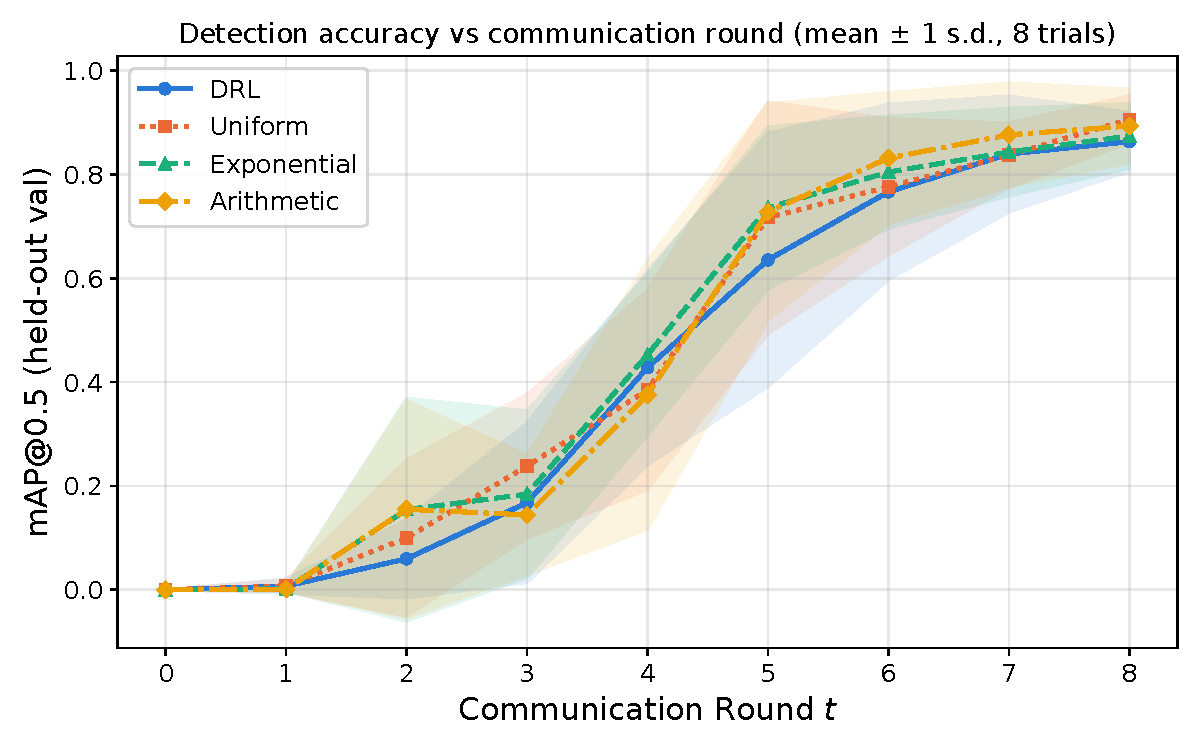
\includegraphics[width=0.9\textwidth]{figA_map_vs_rounds.pdf}
\caption{Detection accuracy against communication round for the learned
allocator and the three fixed baselines, mean over 8 paired trials with $\pm1$
standard deviation bands, scored on held-out data.}
\label{fig:drlmap}
\end{figure}

\begin{figure}[H]
\centering
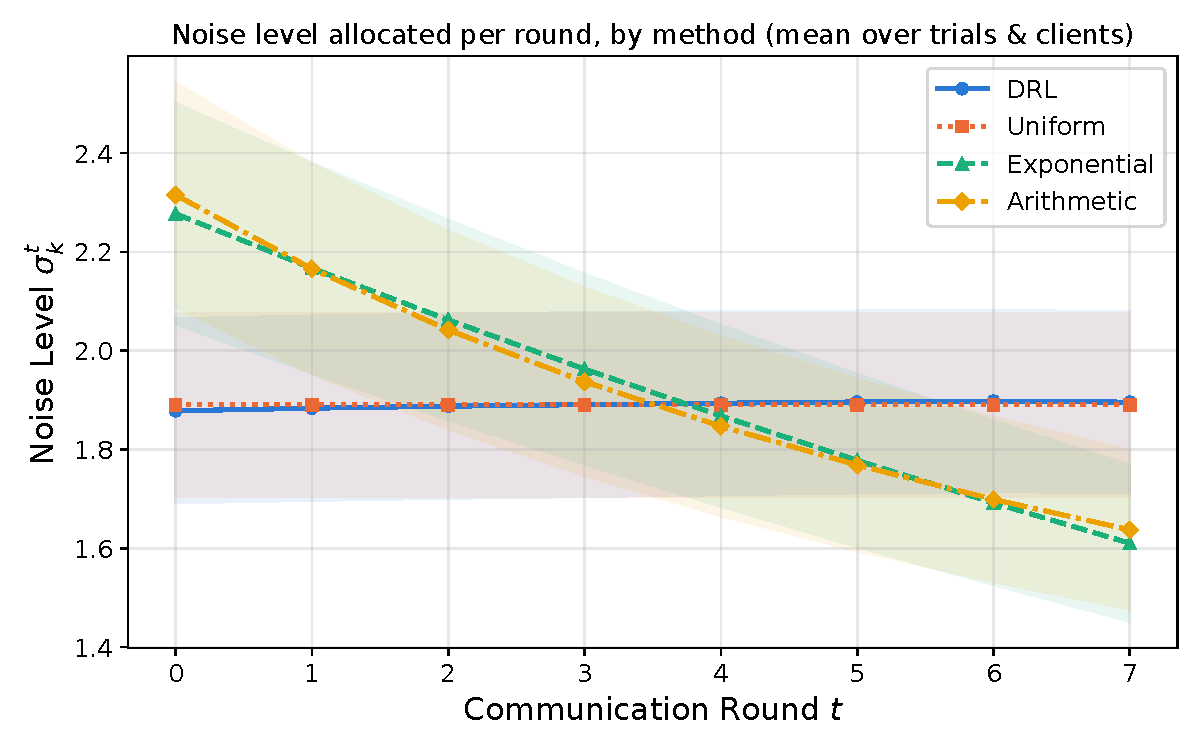
\includegraphics[width=0.9\textwidth]{figB_noise_vs_rounds.pdf}
\caption{The noise schedule the agent actually learned, against the three fixed
schedules. The learned policy is non-uniform, which by
Theorem~\ref{thm:uniform} is the reason it underperforms.}
\label{fig:drlnoise}
\end{figure}

\subsection{A Note on What Is Not Being Claimed}

The single largest effect measured anywhere in this project was a $+0.230$
advantage, $+46\%$ relative, for $T'=6$ at $\rho=0.5$ in the first trial of the
ladder. It did not survive: $n=2$ gave $+0.071$, $n=6$ gave $-0.0003$, and
$n=10$ gave $+0.040$ with 4/10 wins. We report it because it illustrates the
failure mode this chapter is designed to exclude, and because the same
phenomenon plausibly explains small positive results elsewhere in the
literature.

\section{Byzantine Resilience under Differential Privacy}
\label{sec:p3-results}

\subsection{The Honest Update Envelope}
\label{sec:p3-envelope}

Every defence needs a model of what a legitimate update looks like, because that
is what an attacker must imitate, and it is what sets the amplitude an attacker
can use. Table~\ref{tab:envelope} measures it directly.

\begin{table}[H]
\centering
\caption{Honest client update norms. Relative spread collapses once DP noise is
present, matching the $1/\sqrt{2D}=0.094\%$ concentration of a Gaussian norm at
$D=566{,}789$.}
\label{tab:envelope}
\begin{tabular}{lrr}
\toprule
$\sigma$ & Update norm & Relative s.d. \\
\midrule
0 (no DP) & $0.6917\pm0.6548$ & $95\%$ \\
1.83 & $2.2487\pm0.0187$ & $0.83\%$ \\
4.0 & $4.8853\pm0.0095$ & $0.19\%$ \\
8.0 & $9.7586\pm0.0100$ & $0.10\%$ \\
\bottomrule
\end{tabular}
\end{table}

This inverts the premise of DP-exploiting poisoning. Attacks of that family
assume DP noise widens the acceptance band an attacker can hide in. In high
dimensions the norm of a Gaussian vector concentrates, so DP noise makes the
update norm \emph{more} predictable, not less: without noise the norm varies by
$95\%$ across clients, and with it by $0.1\%$, against a theoretical prediction
of $0.094\%$. The camouflage effect is a small-$D$ phenomenon and vanishes at
detector scale.

\vspace{10pt}

What survives is \emph{direction}. A norm detector constrains magnitude only,
and in $566{,}789$ dimensions a rotated update is nearly orthogonal to the
honest one while carrying an indistinguishable norm. We therefore implement the
adaptive attack as a norm-preserving direction attack, which is the strongest
form the envelope permits.

\subsection{Attacks and Defences}

\textbf{RMD} returns a randomly falsified update with no attempt at concealment.
\textbf{$\alpha$-MPELM} steers against the honest update and rescales to the
honest norm, adapting its poisoning degree $\gamma$ according to whether it was
detected in the previous round.

\vspace{10pt}

Defences are a \textbf{norm} detector using a median-absolute-deviation band; an
\textbf{accuracy} detector using server-side validation influence on a held-out
set of 300 frames, disjoint from the 1,200-frame set on which reported metrics
are computed; their \textbf{mix}; and three robust aggregators,
\textbf{Krum} \cite{blanchard2017machine}, \textbf{coordinate-wise median} and
\textbf{trimmed mean} \cite{yin2018byzantine}. The grid comprises 33
configurations $\times$ 3 trials, with 10 clients of 1,904 frames each,
$m\in\{1,2,3\}$ malicious clients, that is $10$ to $30\%$, at $\sigma=1.83$
corresponding to uniform allocation at $\rho=30$, over 15 rounds.

\subsection{Results}

\begin{table}[H]
\centering
\caption{Byzantine resilience at $m=30\%$ malicious clients. IoU$_{.25}$ over
final rounds; TPR is the detection rate against $\alpha$-MPELM; FPR is the
fraction of honest clients wrongly rejected.}
\label{tab:p3}
\begin{tabular}{lrrrrr}
\toprule
Defence & No attack & RMD & $\alpha$-MPELM & TPR & FPR \\
\midrule
None & 0.6485 & 0.6410 & \textbf{0.6312} & --- & 0.00 \\
Norm & 0.6521 & 0.6446 & 0.6428 & 0.14 & 0.10 \\
Accuracy & 0.6656 & 0.6635 & 0.6616 & 0.24 & 0.19 \\
Mix & 0.6655 & 0.6583 & \textbf{0.6649} & \textbf{0.32} & 0.28 \\
Krum & 0.6386 & \textbf{0.5759} & 0.6760 & 0.00 & 0.00 \\
Median & 0.4402 & 0.4333 & \textbf{0.3168} & 0.00 & 0.00 \\
Trimmed mean & 0.6441 & 0.6373 & 0.6282 & 0.00 & 0.00 \\
\bottomrule
\end{tabular}
\end{table}

Three findings follow, illustrated in
Figures~\ref{fig:p1}--\ref{fig:p4}.

\paragraph{The published attack asymmetry reproduces.}
The norm detector catches RMD at a true-positive rate of $1.00$ and
$\alpha$-MPELM at $0.14$. The conventional attack is caught every time and the
adaptive one walks through, which is the headline result of the source work,
reproduced here on a real detector. The episodic adaptation behaves as designed:
$\gamma$ escalates to $1.0$ when the attacker is never caught, and is driven
down to approximately $0.14$ once a detector begins firing
(Figure~\ref{fig:p3}).

\paragraph{The architecture is inherently resilient.}
The worst undefended degradation is $-0.017$ IoU$_{.25}$, or $2.7\%$ relative,
at $30\%$ malicious clients. This follows from the envelope result: with a
roughly $2\%$ norm band an attacker cannot amplify, so the strongest legal move
is direction reversal at matched norm, and three reversed updates in ten merely
scale the average down rather than corrupting its direction. Resilience here is
a \emph{consequence of DP}, not of any defence. Mix detection removes the
residue entirely, scoring $0.6649$ against a $0.6485$ no-attack baseline, at the
cost of rejecting $28\%$ of honest contributions. That trade should be reported
alongside detection rate, since a defence that discards a quarter of legitimate
participants is not free.

\paragraph{Classical robust aggregators are counterproductive under DP.}
Coordinate-wise median costs $-0.208$ IoU$_{.25}$ \emph{with no attacker
present}, an order of magnitude more than any attack studied here, and Krum
costs $-0.073$ under RMD. The reason is structural: averaging is precisely what
suppresses DP noise, by a factor of $\sqrt{N}$, and median and Krum discard that
averaging while also breaking the update's directional structure. Under DP, the
standard Byzantine toolkit can cost more than the threat it addresses. Krum
under $\alpha$-MPELM scores $0.6760$, the highest cell in the table, because
selecting the single most central update happens to exclude direction-reversed
outliers, but the same mechanism loses badly to RMD, so it is not a reliable
defence.

\begin{figure}[H]
\centering
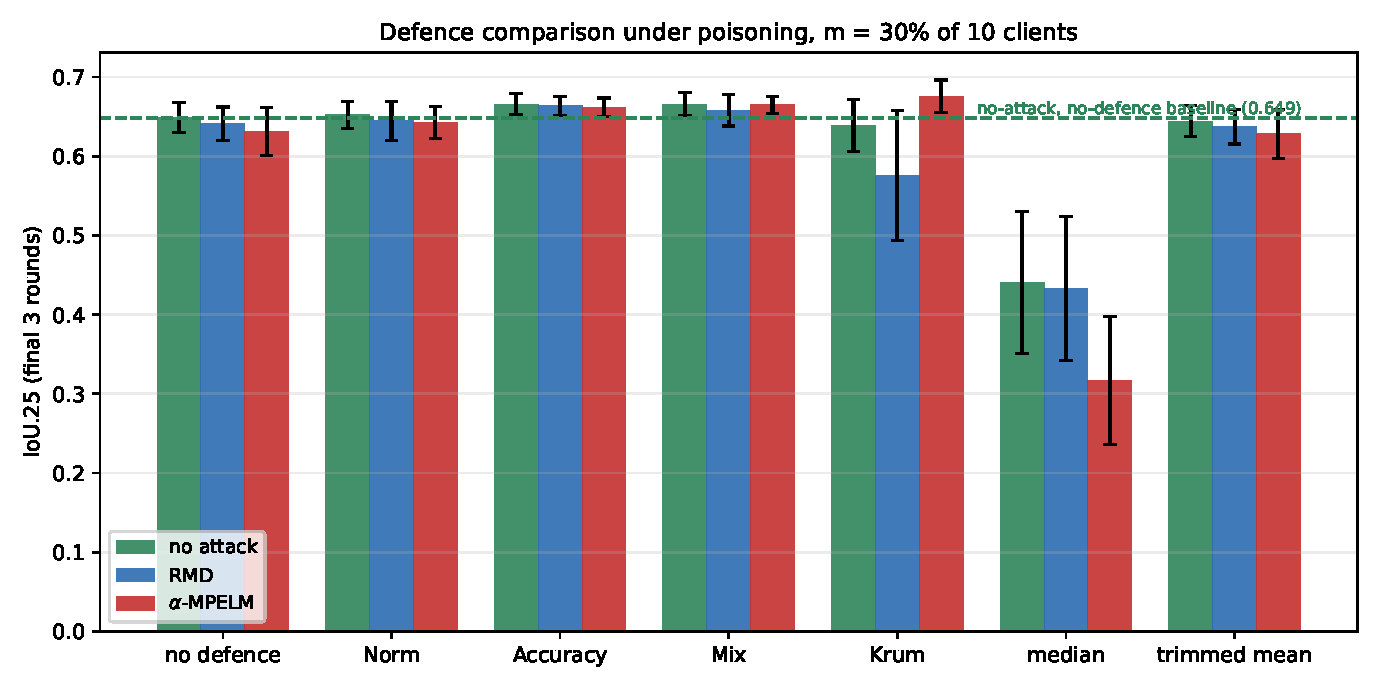
\includegraphics[width=0.95\textwidth]{figP1_defence_comparison.pdf}
\caption{Defence comparison at $m=30\%$ malicious clients.}
\label{fig:p1}
\end{figure}

\begin{figure}[H]
\centering
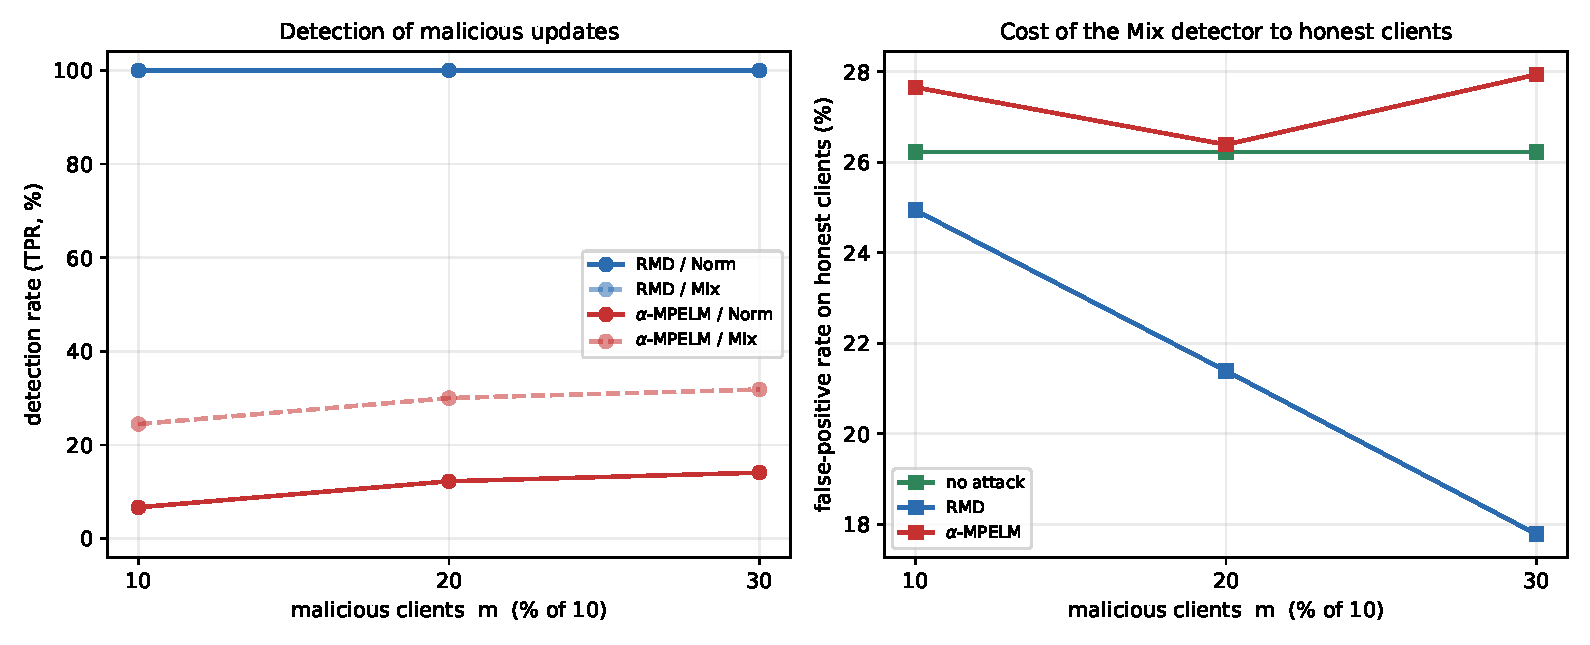
\includegraphics[width=\textwidth]{figP2_detection.pdf}
\caption{Detection rate against malicious ratio, and the false-positive cost
borne by honest clients.}
\label{fig:p2}
\end{figure}

\begin{figure}[H]
\centering
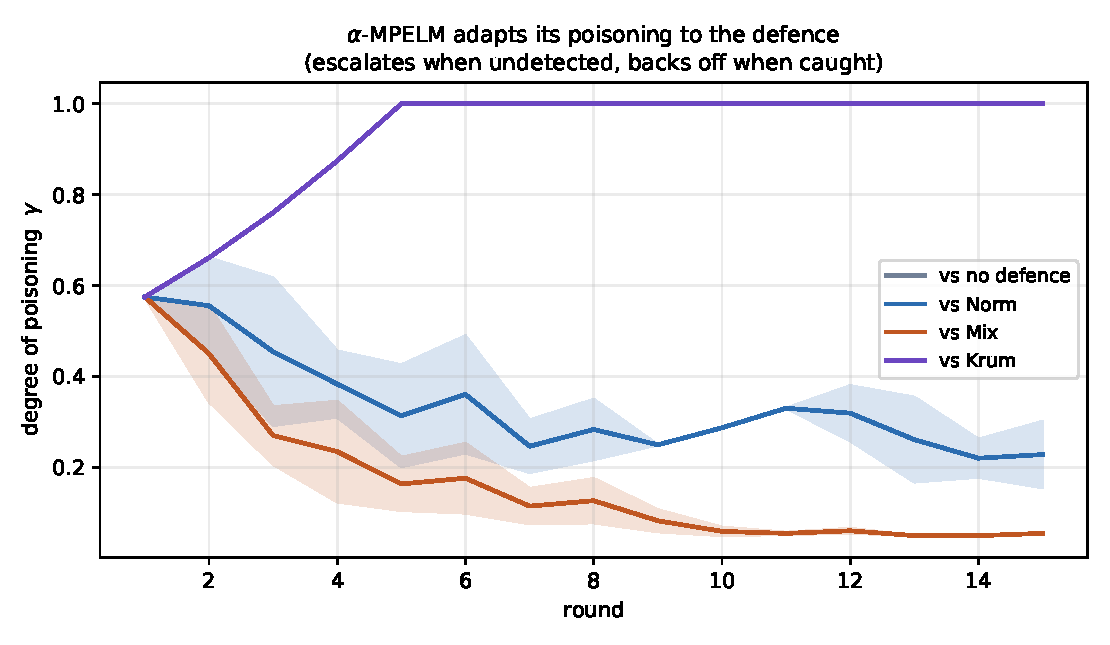
\includegraphics[width=0.75\textwidth]{figP3_gamma.pdf}
\caption{Poisoning degree $\gamma$ over rounds: the attacker escalates when
undetected and retreats when caught.}
\label{fig:p3}
\end{figure}

\begin{figure}[H]
\centering
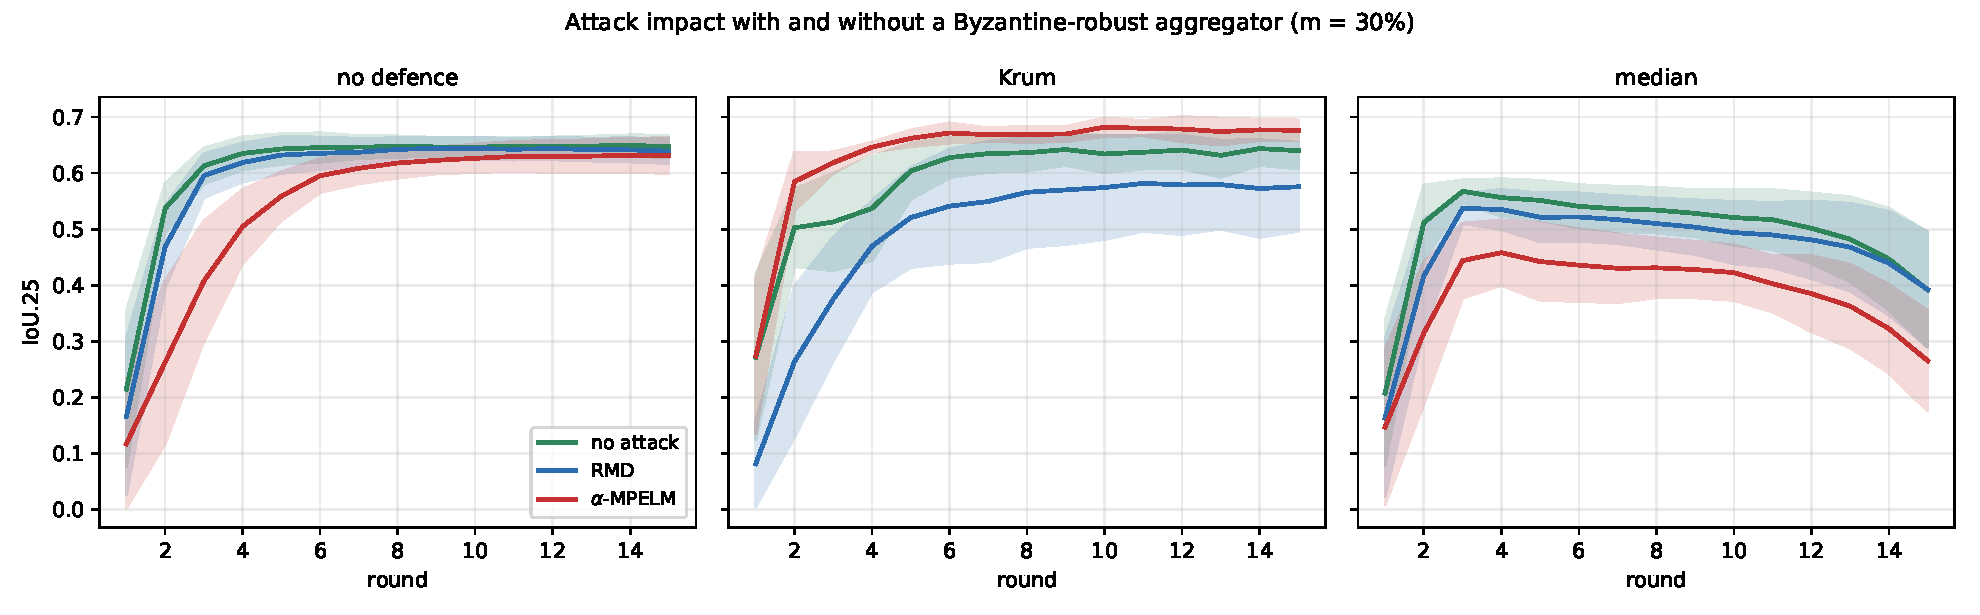
\includegraphics[width=\textwidth]{figP4_robust_agg.pdf}
\caption{Accuracy trajectories with and without robust aggregation.}
\label{fig:p4}
\end{figure}
